\documentclass{beamer}
\usetheme{CambridgeUS}
\title[Process]{The Koopman operator}
\subtitle{Nonlinear MPC + Kalman Filter}
\institute[Polimi]{Politecnico di Milano}
\author{Sergio Vanegas}
\date{\today}

\usepackage{listings}

\usepackage{caption}
\usepackage{subcaption}
\usepackage{dirtytalk}

\usepackage{graphicx}

\usepackage{siunitx}

\begin{document}

\begin{frame}[plain,noframenumbering]
    \maketitle
\end{frame}

\begin{frame}{Table of Contents}
    \tableofcontents
\end{frame}


\section{Introduction}

\begin{frame}{Introduction}
    In this presentation we present the final version of the nonlinear MPC for the Van Der Pol oscillator that will be used as reference from now on, and then proceed to evaluate different methodologies to replicate its behaviour using the Koopman operator.

    We start by defining the nonlinear MPC, simulation parameters and data format for replicability's sake.

    Then, we introduce the memory-reliant Koopman controller, basing the amount of stored samples on the Control Horizon parameter of the reference MPC. In this section we also compare its performance to the (polished) memoryless implementation discussed last meeting.

    After that, we introduce the Kalman-informed framework from which we will repeat the Koopman identification process, including the memoryless vs memory-reliant comparison.

    Finally, we will present the conclusions based on the overall results and determine the best implementation for each scenario.
\end{frame}


\section{Reference controller}

\begin{frame}{Nonlinear MPC - Parameters}
    \begin{itemize}
        \item Sampling time: $0.01$ seconds
        \item Total simulation time: $2000$ seconds
        \item Number of I/O: 2/2 (identity relationship)
        \item Internal model sub-step: 10 steps $\rightarrow 0.001$ seconds
        \item Prediction horizon: 15 samples $\rightarrow 0.15$ seconds
        \item Control horizon: 3 samples $\rightarrow 0.03$ seconds
        \item Output variables' weights: $\left[1.0 \quad 0.0\right]$
        \item Second state boundaries: $\left[-1.0 \quad 1.0\right]$
    \end{itemize}

    Once again, we use the Van der Pol simulations as reference. We remove the integrator block reset signal since we are now sure the controller is stable (first-state control + second-state boundaries).
\end{frame}

\begin{frame}{Simulink model - Reference}
    \begin{figure}
        \centering
        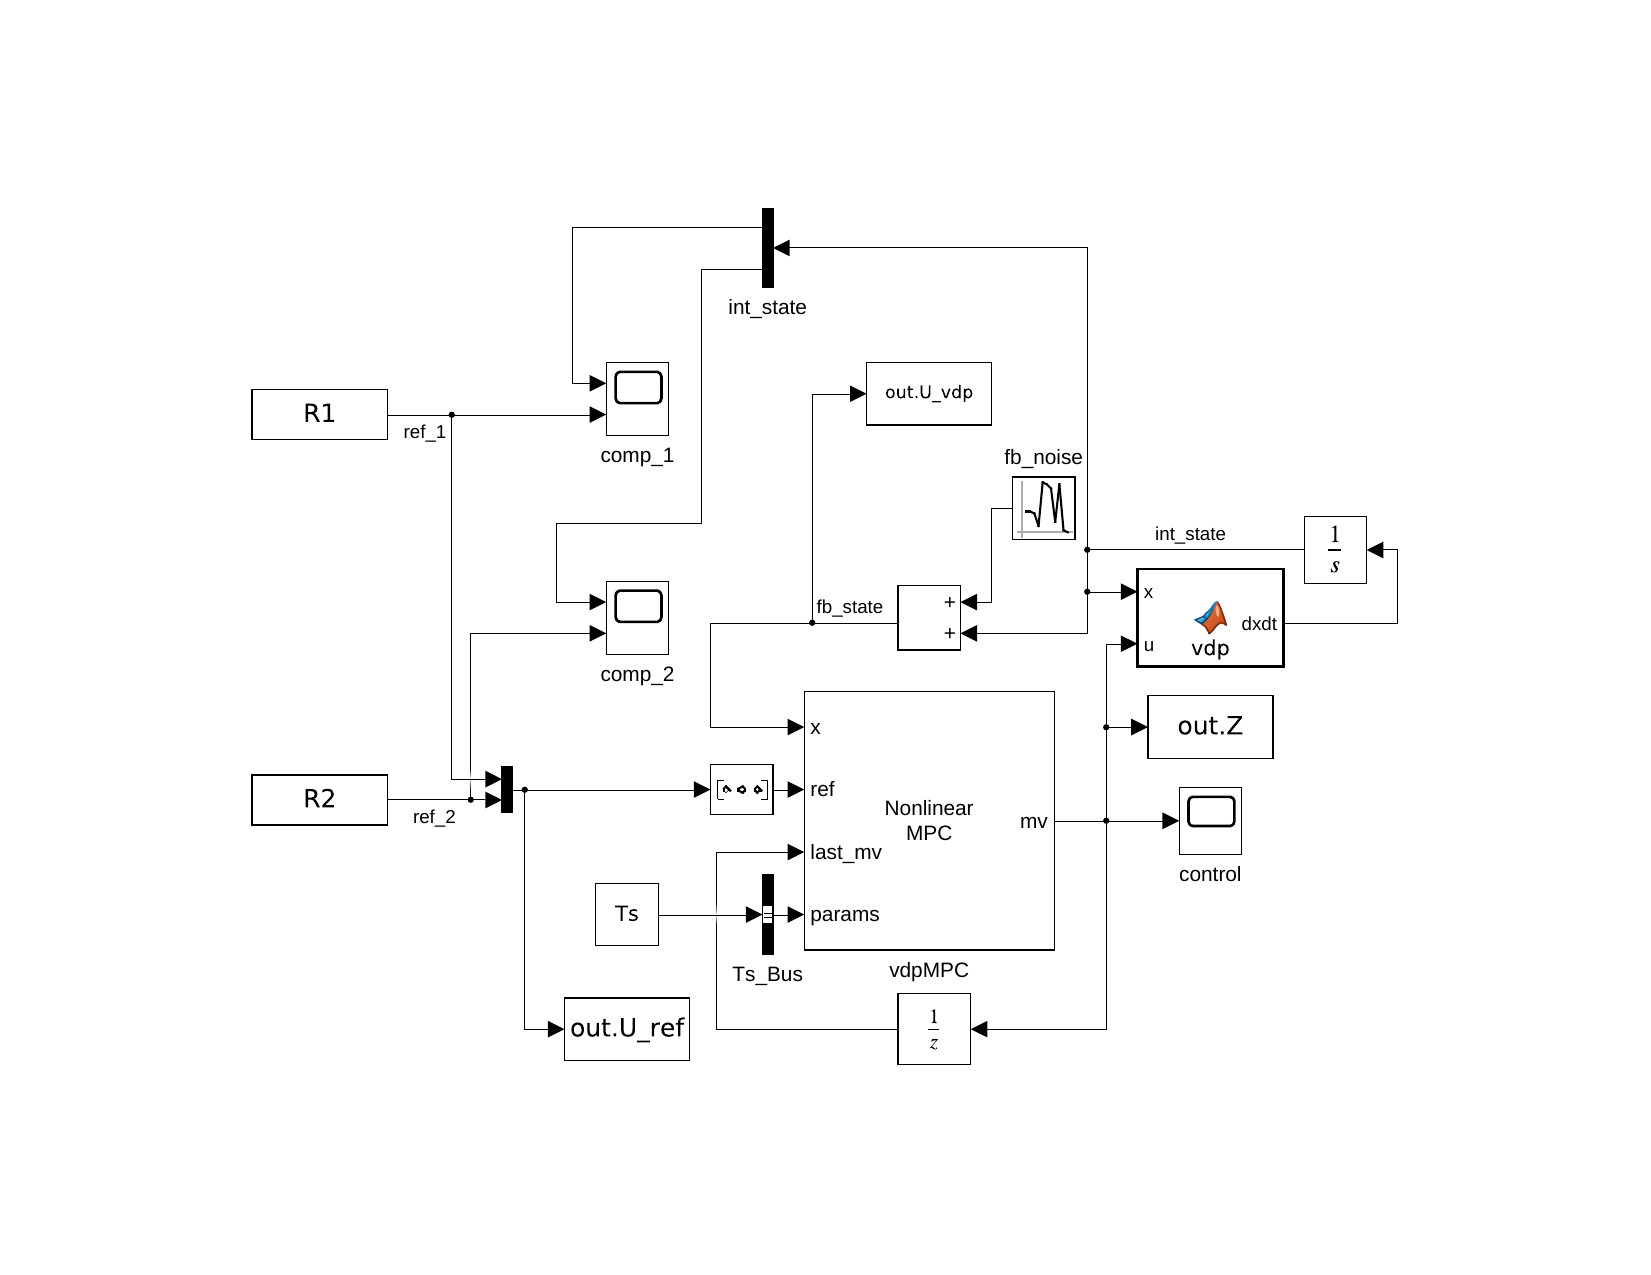
\includegraphics[width=0.75\textwidth]{Simulink_VDP.png}
    \end{figure}
\end{frame}


\section{Koopman controller}

\begin{frame}{Nonlinear Koopman controller - Parameters}
    Since we are now only predicting the immediately successive state instead of the whole observable collection, we have a lot more freedom regarding the number of observables and the dataset size used during the identification algorithm.

    \begin{itemize}
        \item Number of observables: 25
        \item Input type: hybrid (reference, noisy measured states and their difference)
        \item Regularization coefficient: $0.001$
        \item Longest delay: $z^{-2}$
    \end{itemize}

    Given the non-linearity of the new implementation, the matrix multiplications and ZOH's had to be implemented manually, fitting the observable function inside the delayed feedback loop. The $L^2$ error was calculated w.r.t. the noiseless signals.
\end{frame}

\begin{frame}{Simulink model - Benchmark}
    \begin{figure}
        \centering
        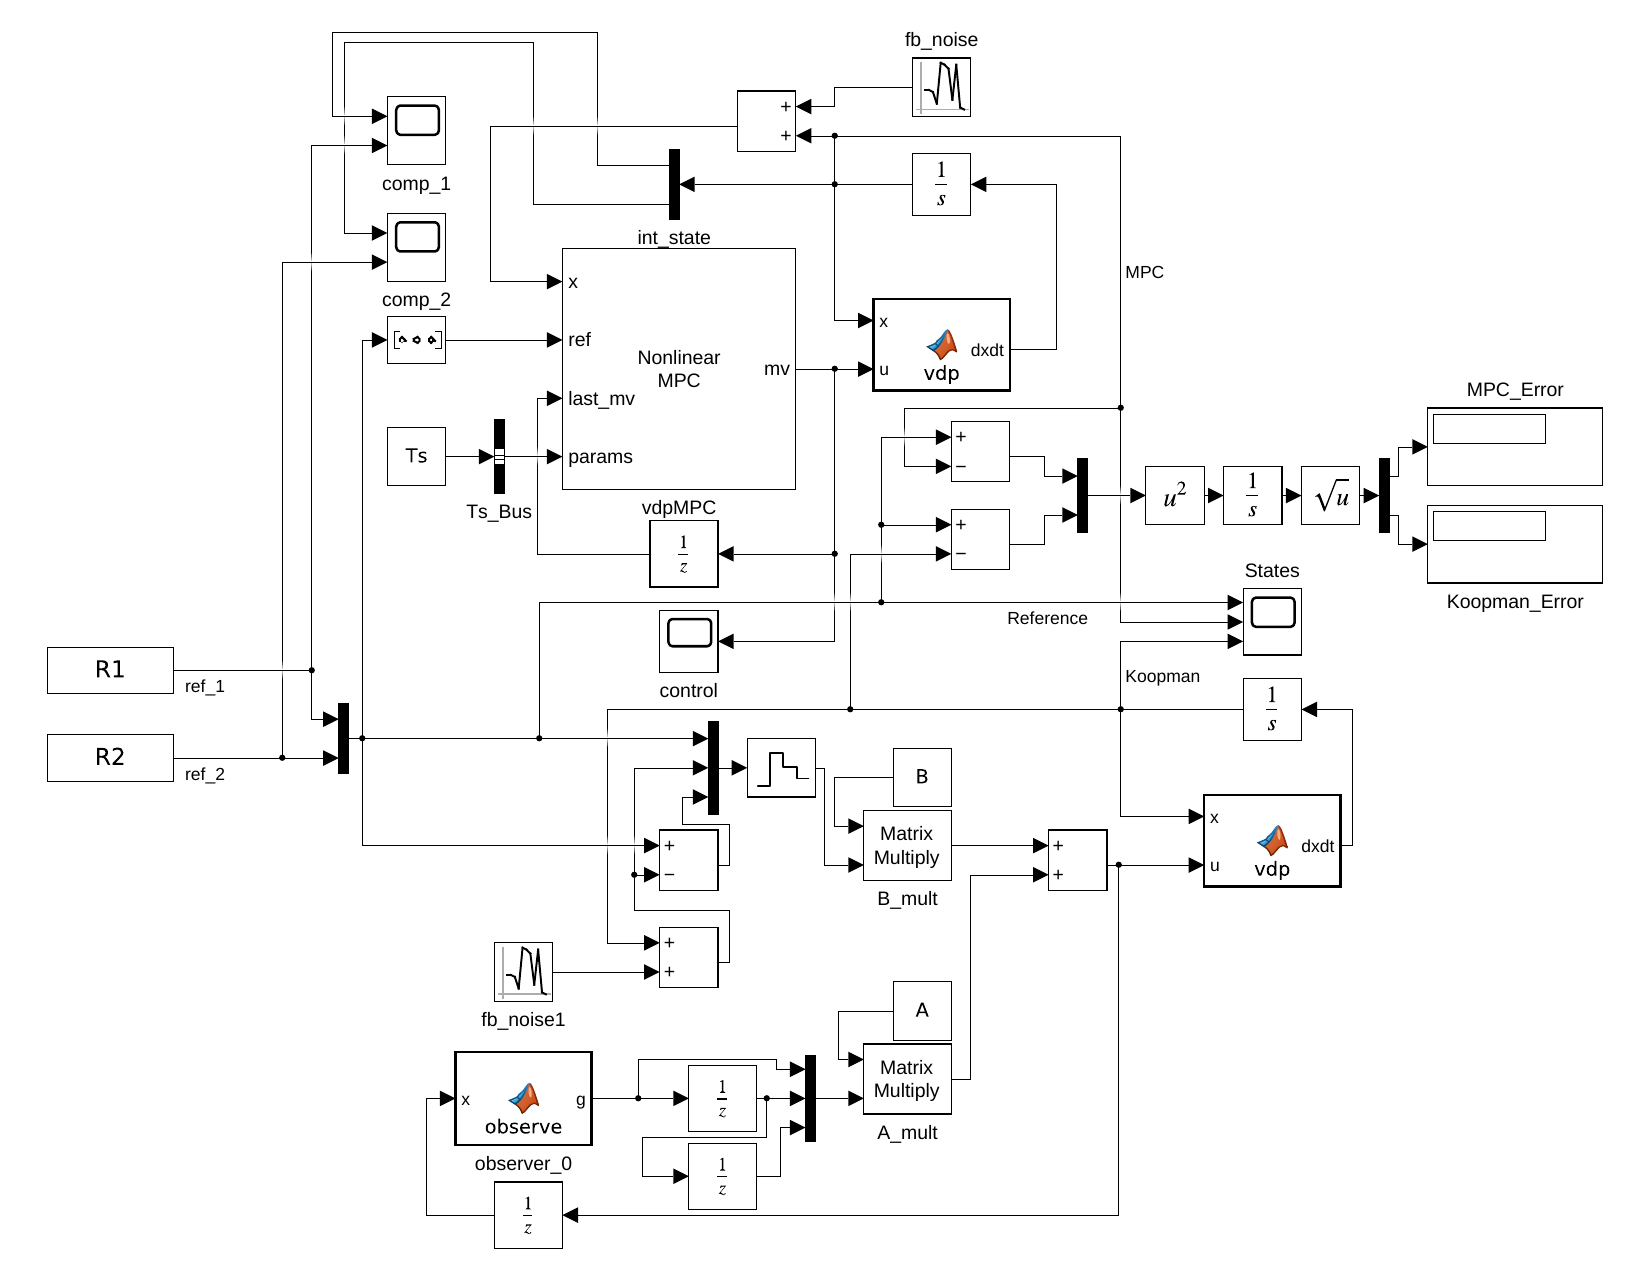
\includegraphics[width=0.75\textwidth]{Simulink_Koopman.png}
    \end{figure}
\end{frame}

\begin{frame}{Nonlinear Koopman controller - Numerical results}
    We numerically compare the performance of the controllers by observing their $L^2$ error throughout a $20$ second\footnote{time-frame selected based on the duration of the recorded trajectories} over three different references.

    \begin{itemize}
        \item Impulse error (single sample, second-state reference equal to 0)
            \begin{itemize}
                \item MPC $\rightarrow \left(0.114,0.353\right)$
                \item Memoryless Koopman $\rightarrow \left(0.105,0.082\right)$
                \item Memory-reliant Koopman $\rightarrow \left(0.106,0.087\right)$
            \end{itemize}
        \item Step error ($@t=0.0$, second-state reference equal to 0)
            \begin{itemize}
                \item MPC $\rightarrow \left(0.450,0.705\right)$
                \item Memoryless Koopman $\rightarrow \left(0.559,0.623\right)$
                \item Memory-reliant Koopman $\rightarrow \left(0.556,0.639\right)$
            \end{itemize}
        \item Trajectory error (non-convergent reference)
            \begin{itemize}
                \item MPC $\rightarrow \left(0.352,0.649\right)$
                \item Memoryless Koopman $\rightarrow \left(0.486,0.477\right)$
                \item Memory-reliant Koopman $\rightarrow \left(0.490,0.511\right)$
            \end{itemize}
    \end{itemize}
\end{frame}

\begin{frame}{Nonlinear Koopman controller - Impulse response}
    \begin{figure}
        \centering
        \begin{subfigure}[b]{0.45\textwidth}
            \centering
            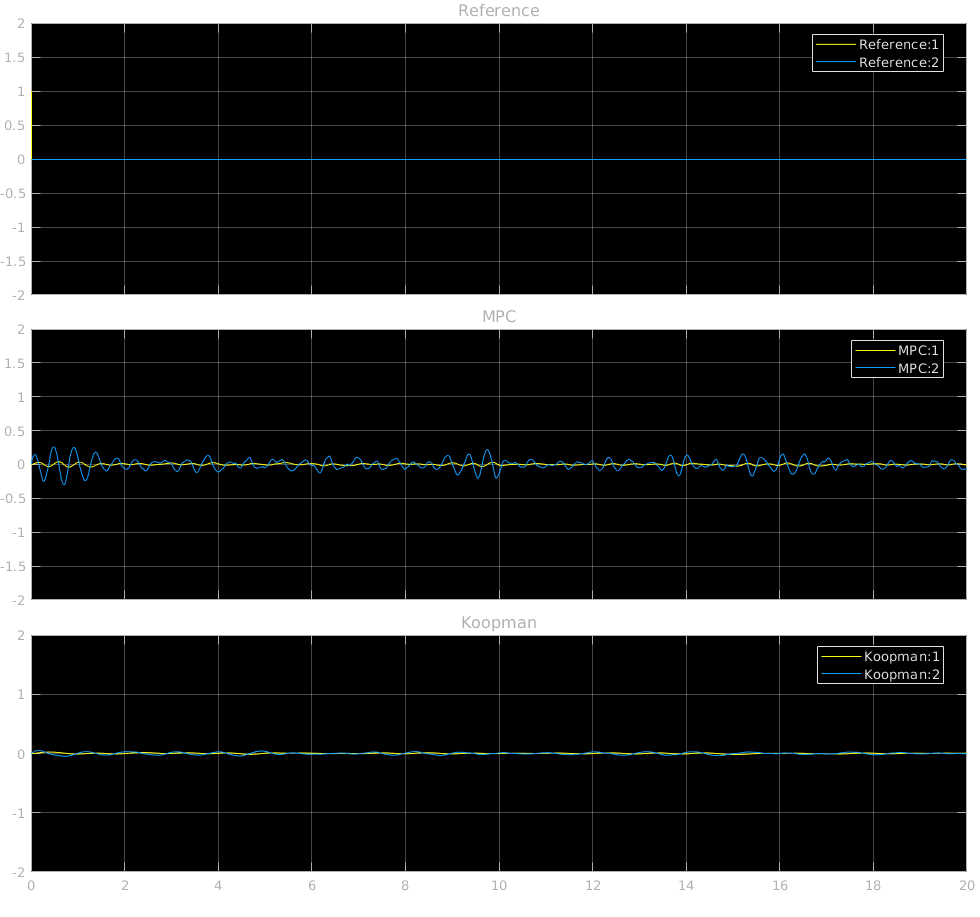
\includegraphics[width=\textwidth]{Undelayed_Koopman_Pulse.png}
            \caption{Memoryless controller}
        \end{subfigure}
        \hfill
        \begin{subfigure}[b]{0.45\textwidth}
            \centering
            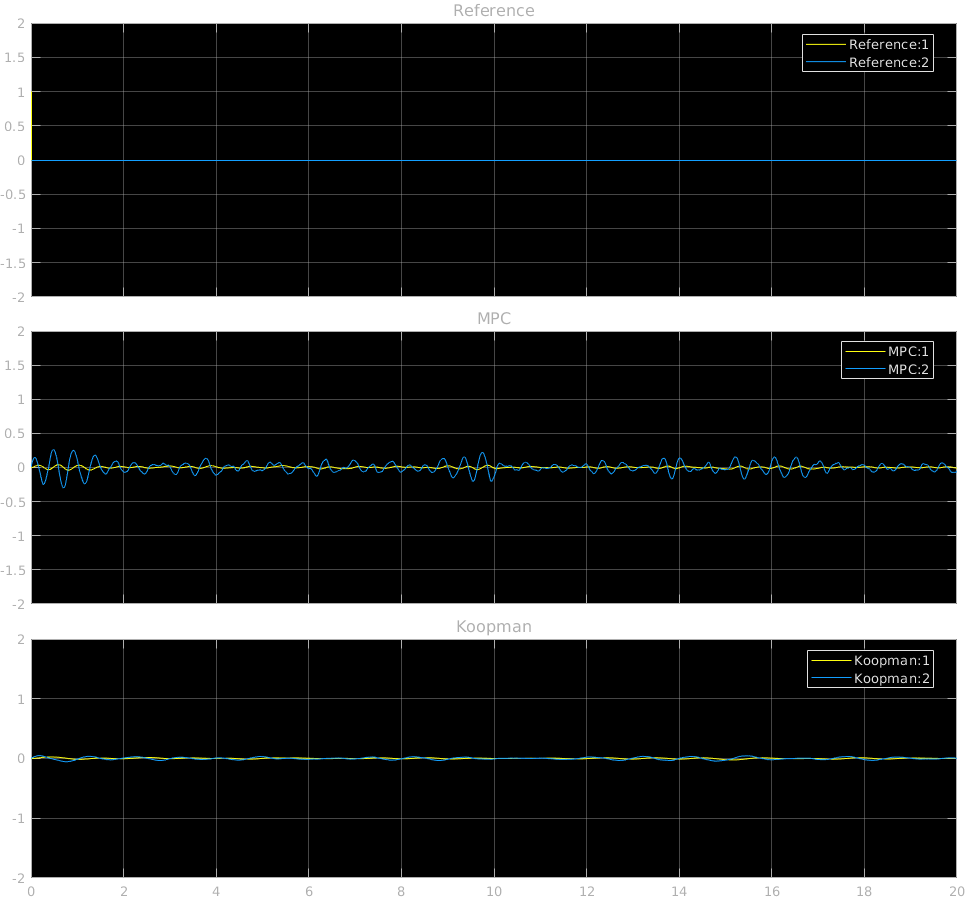
\includegraphics[width=\textwidth]{Delayed_Koopman_Pulse.png}
            \caption{Memory-reliant controller}
        \end{subfigure}
    \end{figure}
\end{frame}

\begin{frame}{Nonlinear Koopman controller - Step response}
    \begin{figure}
        \centering
        \begin{subfigure}[b]{0.45\textwidth}
            \centering
            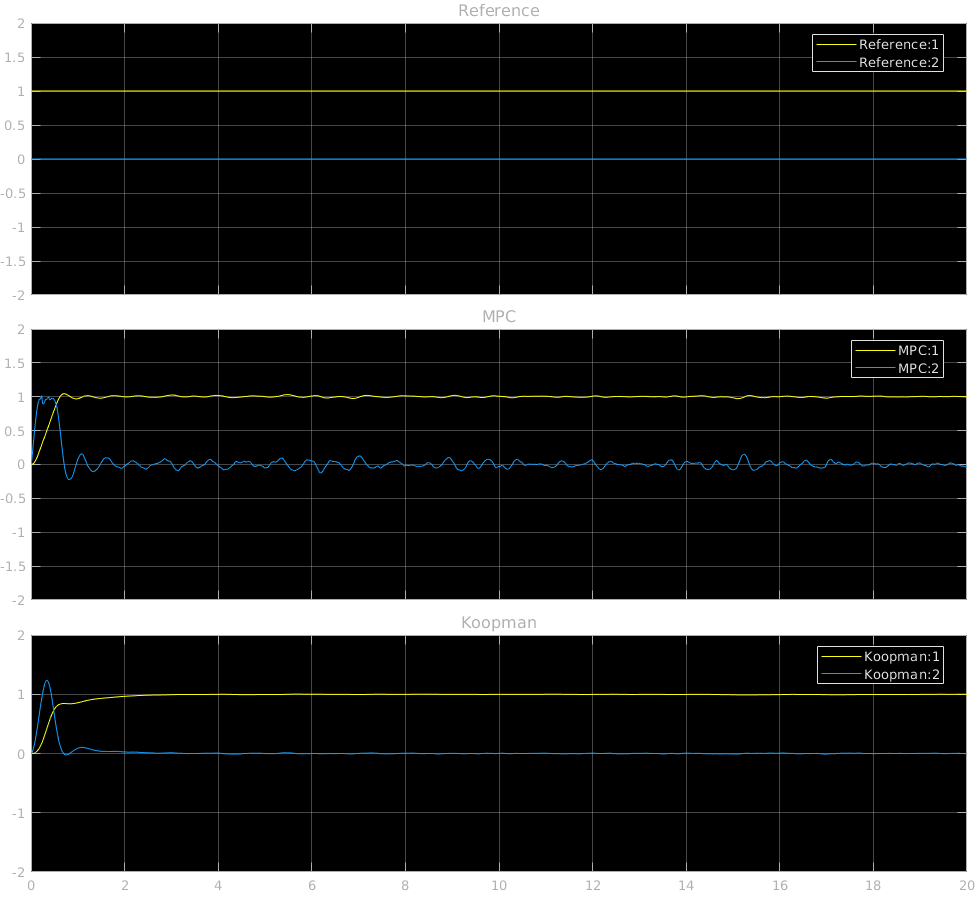
\includegraphics[width=\textwidth]{Undelayed_Koopman_Step.png}
            \caption{Memoryless controller}
        \end{subfigure}
        \hfill
        \begin{subfigure}[b]{0.45\textwidth}
            \centering
            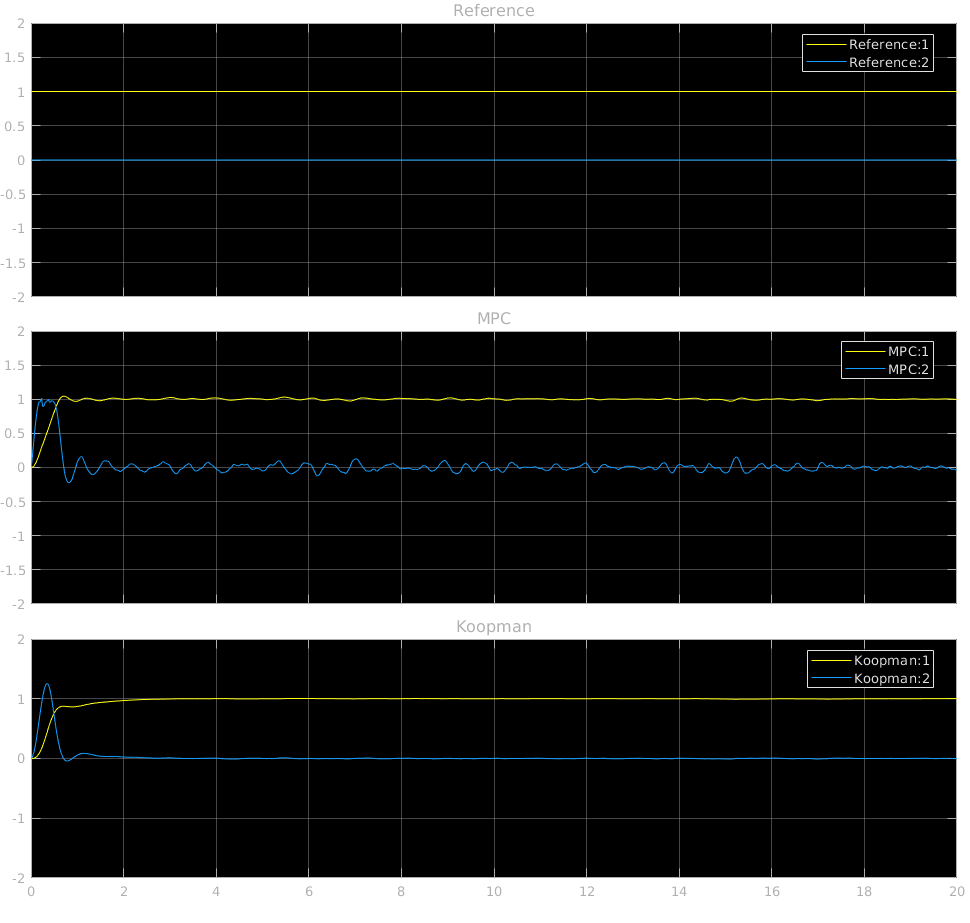
\includegraphics[width=\textwidth]{Delayed_Koopman_Step.png}
            \caption{Memory-reliant controller}
        \end{subfigure}
    \end{figure}
\end{frame}

\begin{frame}{Nonlinear Koopman controller - Trajectory tracking}
    \begin{figure}
        \centering
        \begin{subfigure}[b]{0.45\textwidth}
            \centering
            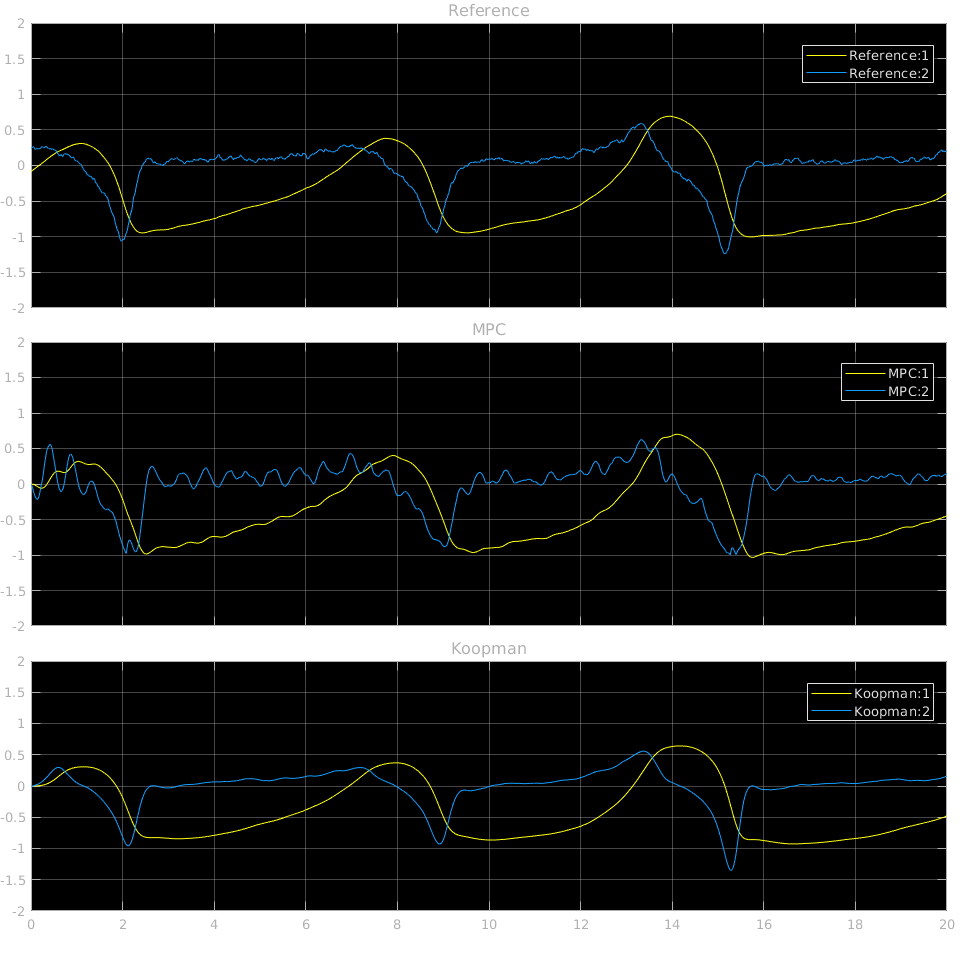
\includegraphics[width=\textwidth]{Undelayed_Koopman_Ref.png}
            \caption{Memoryless controller}
        \end{subfigure}
        \hfill
        \begin{subfigure}[b]{0.45\textwidth}
            \centering
            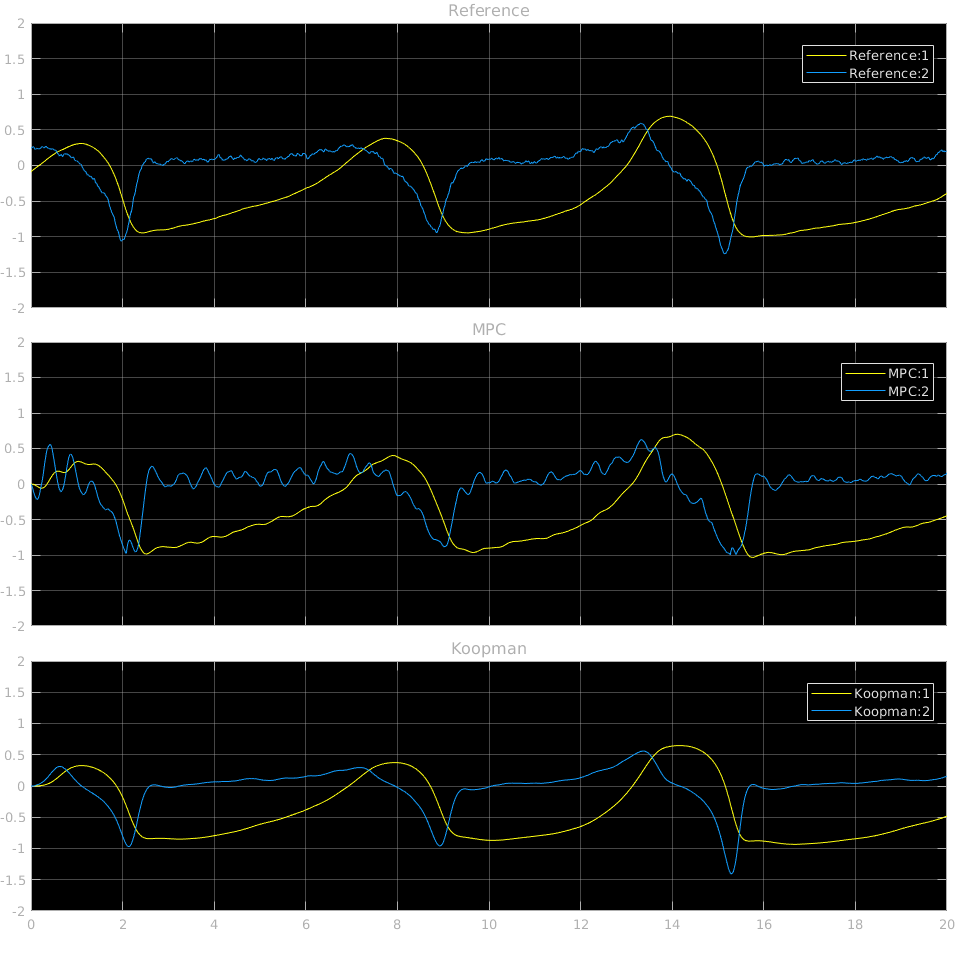
\includegraphics[width=\textwidth]{Delayed_Koopman_Ref.png}
            \caption{Memory-reliant controller}
        \end{subfigure}
    \end{figure}
\end{frame}


\section{Kalman-informed Koopman controller}

\begin{frame}{Kalman-informed MPC - Considerations}
    \begin{itemize}
        \item Same MPC controller parameters
        \item Kalman filter fed-back with the noisy measured first state (measure function represented by matrix $\left[1 \quad 0\right]$)
        \item Jacobian generated by interpreting the forward-Euler scheme as a single sub-step operation
        \item 0 variance inside the state function; all noise is considered to come from the measurement function
        \item We keep using the Van der Pol clean simulations as reference.
    \end{itemize}
\end{frame}

\begin{frame}{Simulink model - Reference}
    \begin{figure}
        \centering
        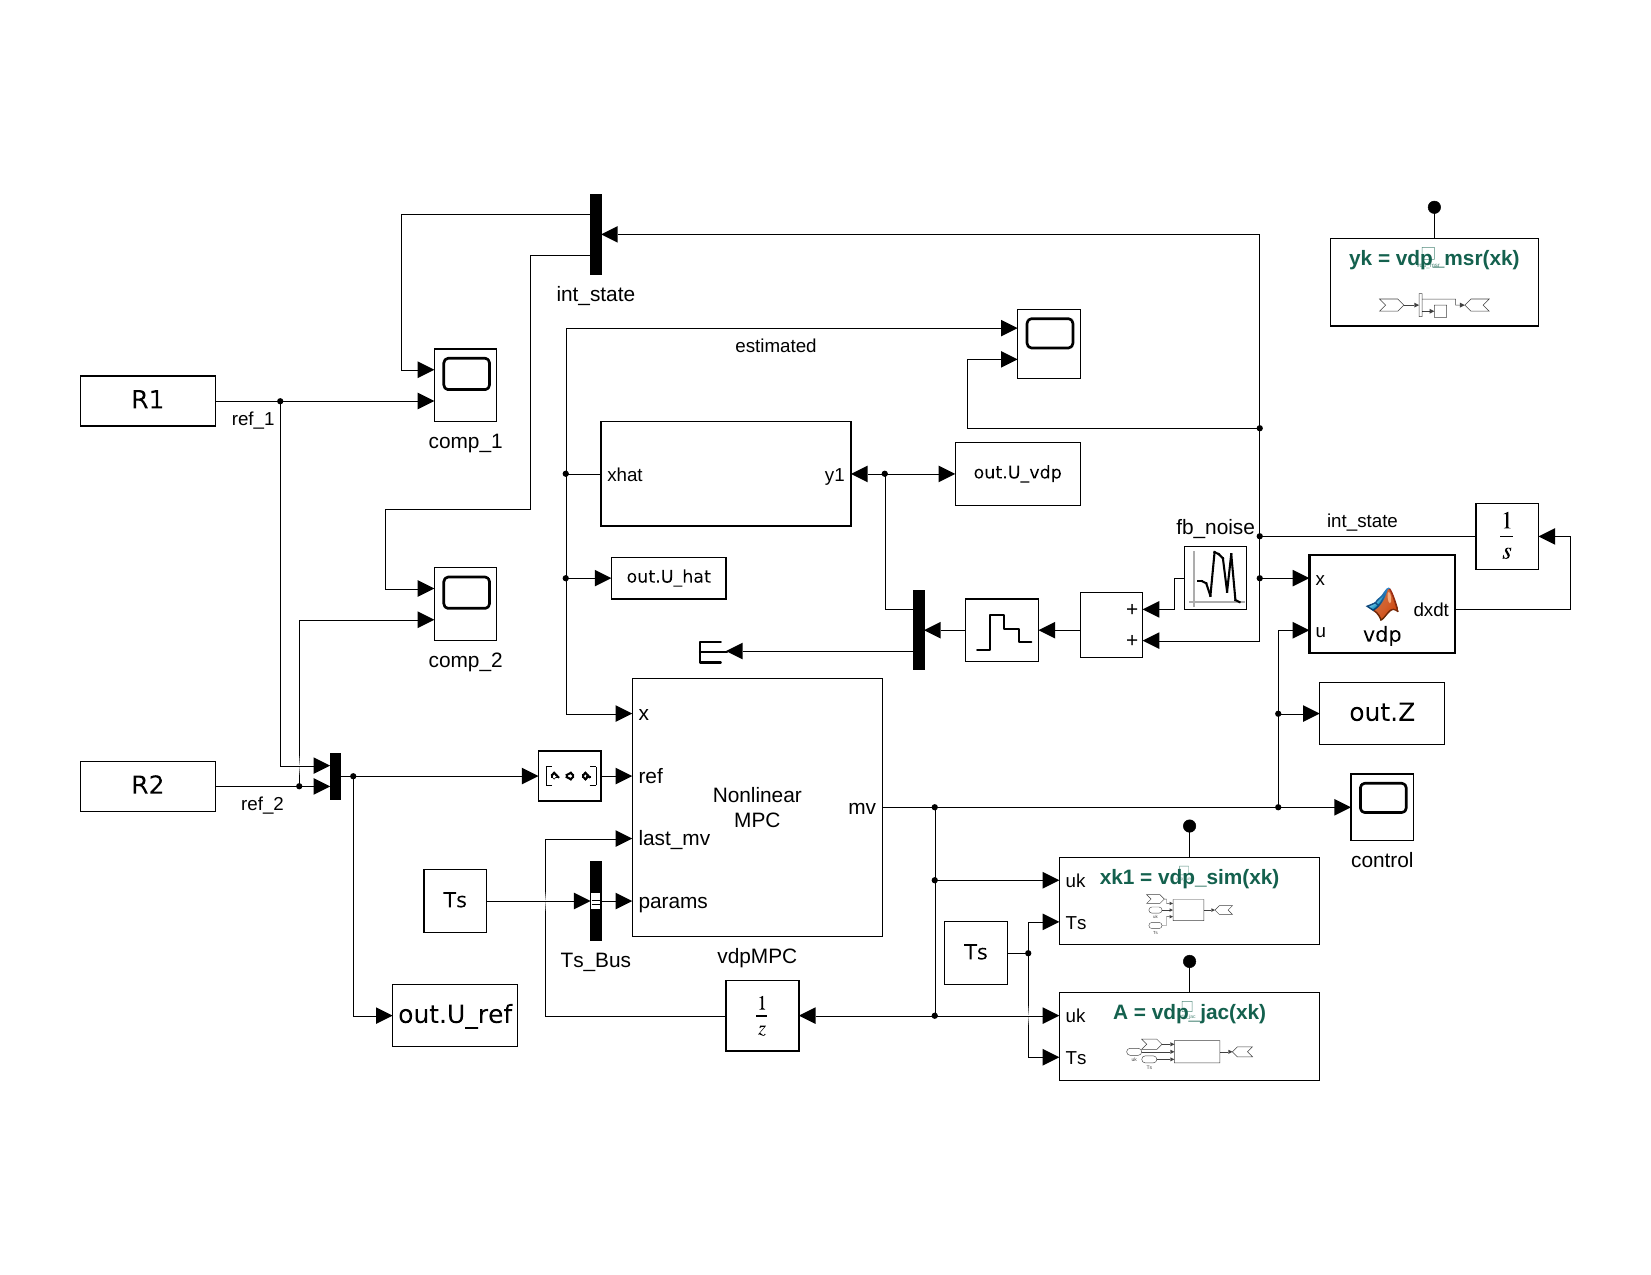
\includegraphics[width=0.75\textwidth]{Simulink_Kalman.png}
    \end{figure}
\end{frame}

\begin{frame}{Kalman-Koopman controller - Parameters}
    A similar pipeline was intended for the Kalman-informed Koopman controller. Nevertheless, a memory-reliant version could not be evaluated, since no combination of parameters stabilized the controller (memory size for both input and output, regularization coefficient, etc). Therefore, different observable collections were compared in its stead.

    \begin{itemize}
        \item Number of observables: 10/20/50
        \item Input type: hybrid (reference, noisy first measured state and its difference)
        \item Regularization coefficient: 0.001
    \end{itemize}
\end{frame}

\begin{frame}{Simulink model - Benchmark}
    \begin{figure}
        \centering
        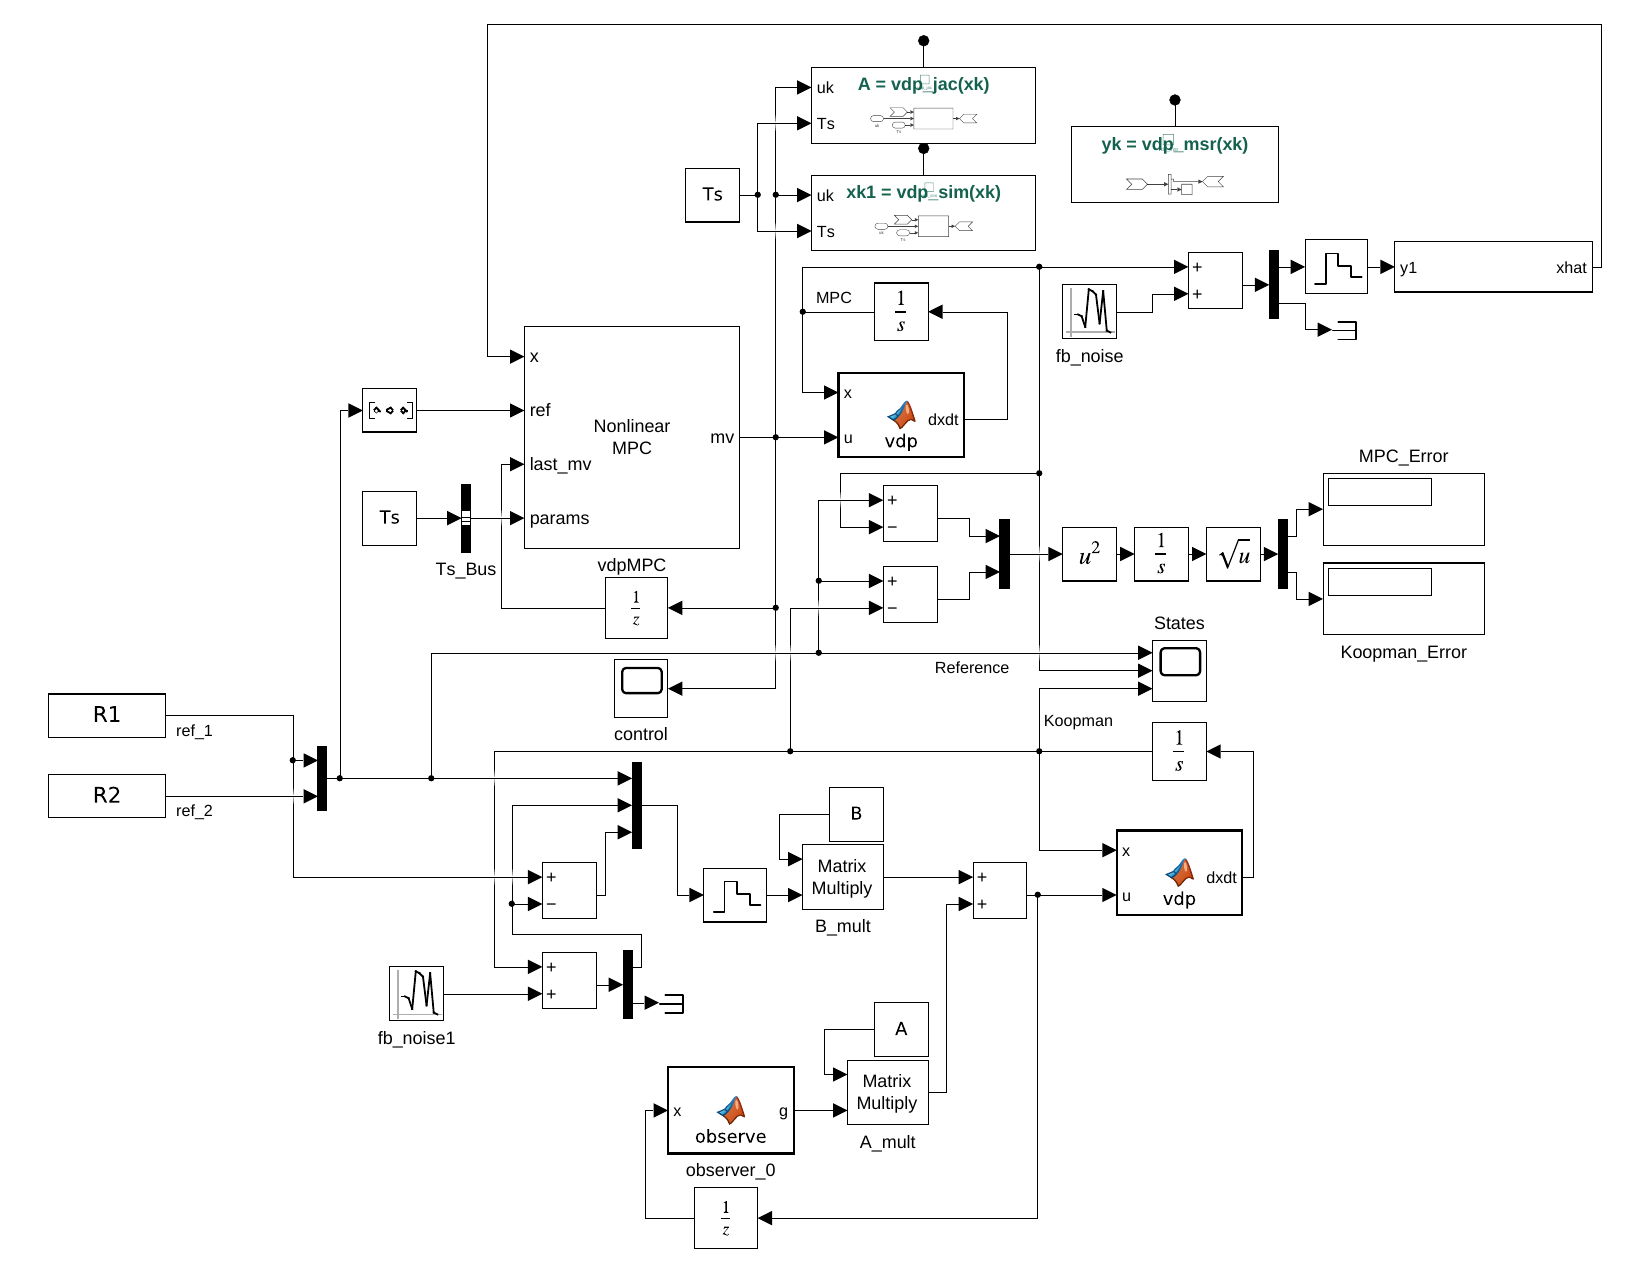
\includegraphics[width=0.75\textwidth]{Simulink_KK.png}
    \end{figure}
\end{frame}

\begin{frame}[allowframebreaks]{Kalman-Koopman controller - Numerical results}
    We repeat the numerical benchmark used for the Nonlinear Koopman controller but, as mentioned before, we compare different library sizes instead of memoryless vs memory-reliant.

    \begin{itemize}
        \item Impulse error (single sample, second-state reference equal to 0)
            \begin{itemize}
                \item Kalman-MPC $\rightarrow \left(0.114,0.269\right)$
                \item 10 observables $\rightarrow \left(2.759,1.944\right)$
                \item 20 observables $\rightarrow \left(2.763,1.950\right)$
                \item 50 observables $\rightarrow \left(2.780,1.972\right)$
            \end{itemize}
        \item Step error ($@t=0.0$, second-state reference equal to 0)
            \begin{itemize}
                \item Kalman-MPC $\rightarrow \left(0.496,0.694\right)$
                \item 10 observables $\rightarrow \left(1.833,0.401\right)$
                \item 20 observables $\rightarrow \left(1.882,0.401\right)$
                \item 50 observables $\rightarrow \left(1.873,0.402\right)$
            \end{itemize}
        \item Trajectory error (non-convergent reference)
            \begin{itemize}
                \item Kalman-MPC $\rightarrow \left(0.333,0.534\right)$
                \item 10 observables $\rightarrow \left(2.895,2.215\right)$
                \item 20 observables $\rightarrow \left(2.808,2.178\right)$
                \item 50 observables $\rightarrow \left(2.766,2.156\right)$
            \end{itemize}
    \end{itemize}
\end{frame}

\begin{frame}{Kalman-Koopman controller - Impulse response}
    \begin{figure}
        \centering
        \begin{subfigure}[b]{0.3\textwidth}
            \centering
            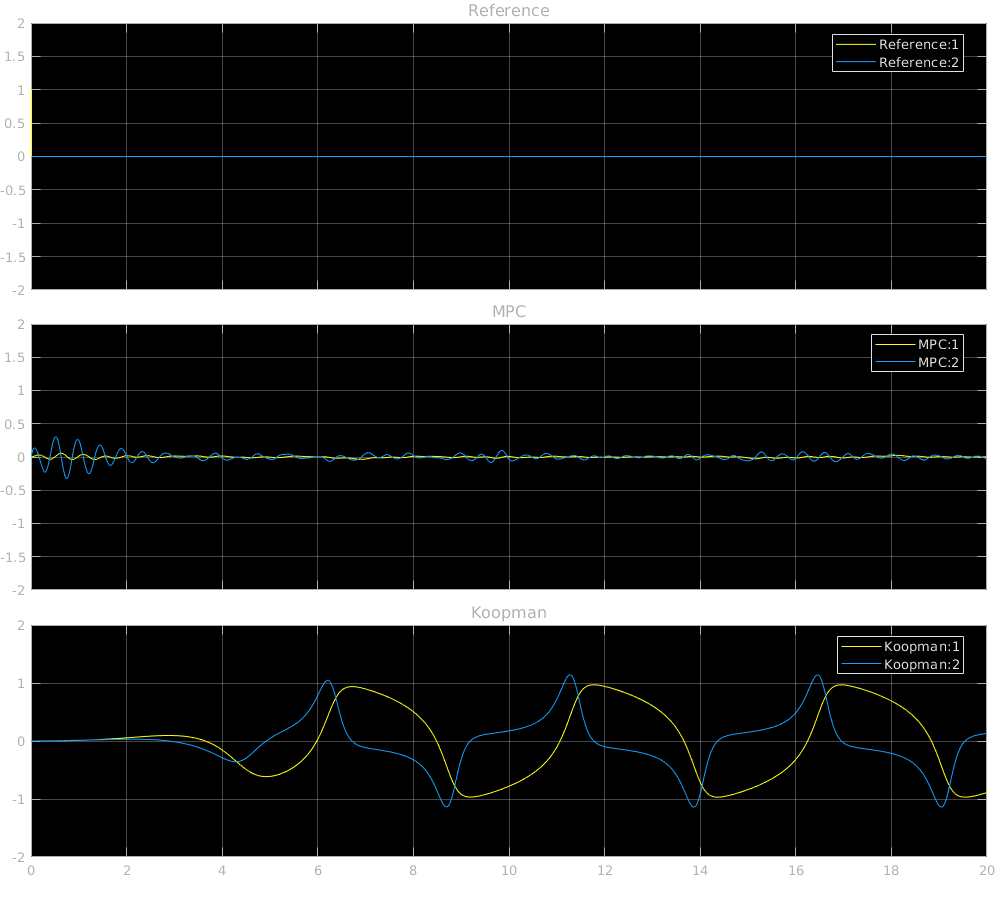
\includegraphics[width=\textwidth]{KK_10_Pulse.png}
            \caption{10 functions}
        \end{subfigure}
        \hfill
        \begin{subfigure}[b]{0.3\textwidth}
            \centering
            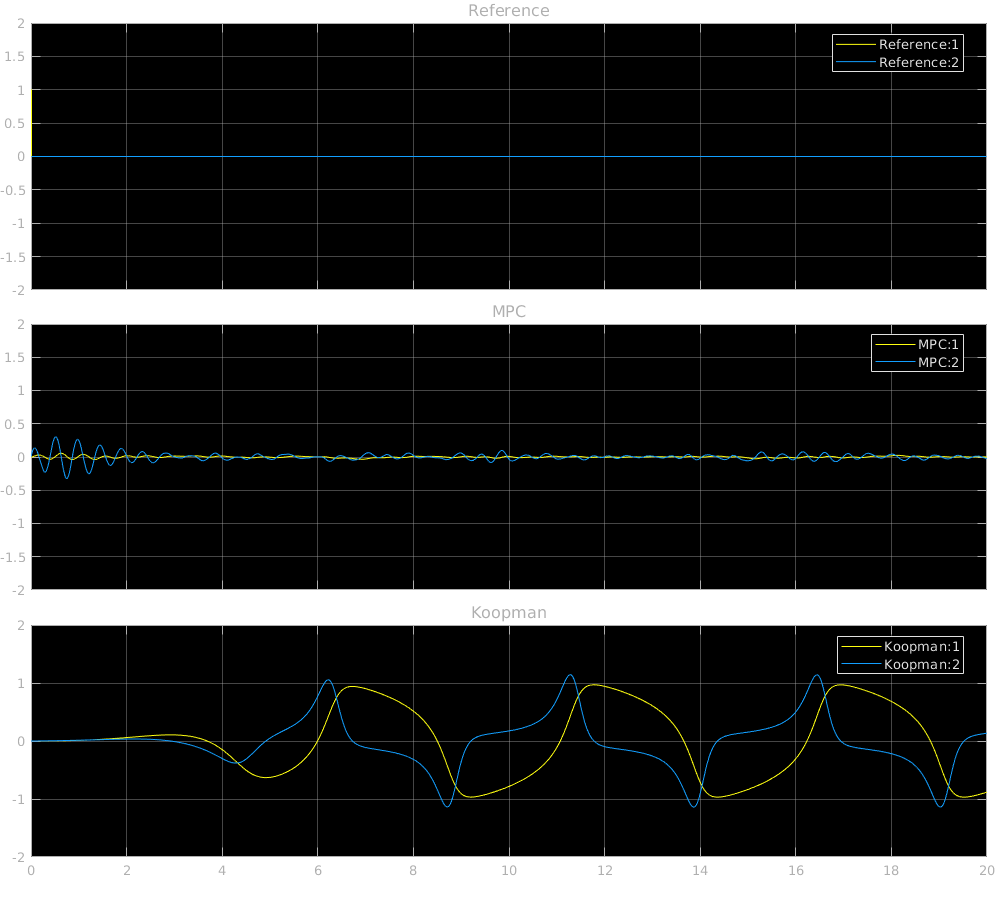
\includegraphics[width=\textwidth]{KK_20_Pulse.png}
            \caption{20 functions}
        \end{subfigure}
        \hfill
        \begin{subfigure}[b]{0.3\textwidth}
            \centering
            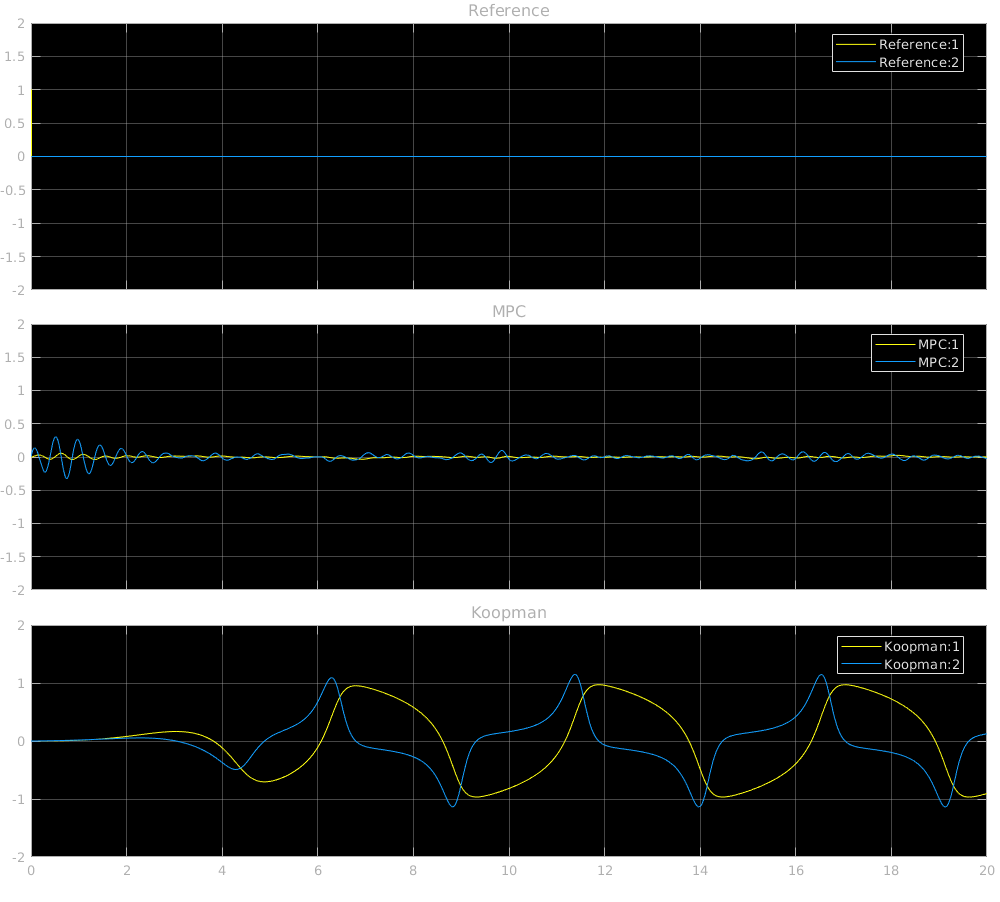
\includegraphics[width=\textwidth]{KK_50_Pulse.png}
            \caption{50 functions}
        \end{subfigure}
    \end{figure}
\end{frame}

\begin{frame}{Kalman-Koopman controller - Step response}
    \begin{figure}
        \centering
        \begin{subfigure}[b]{0.3\textwidth}
            \centering
            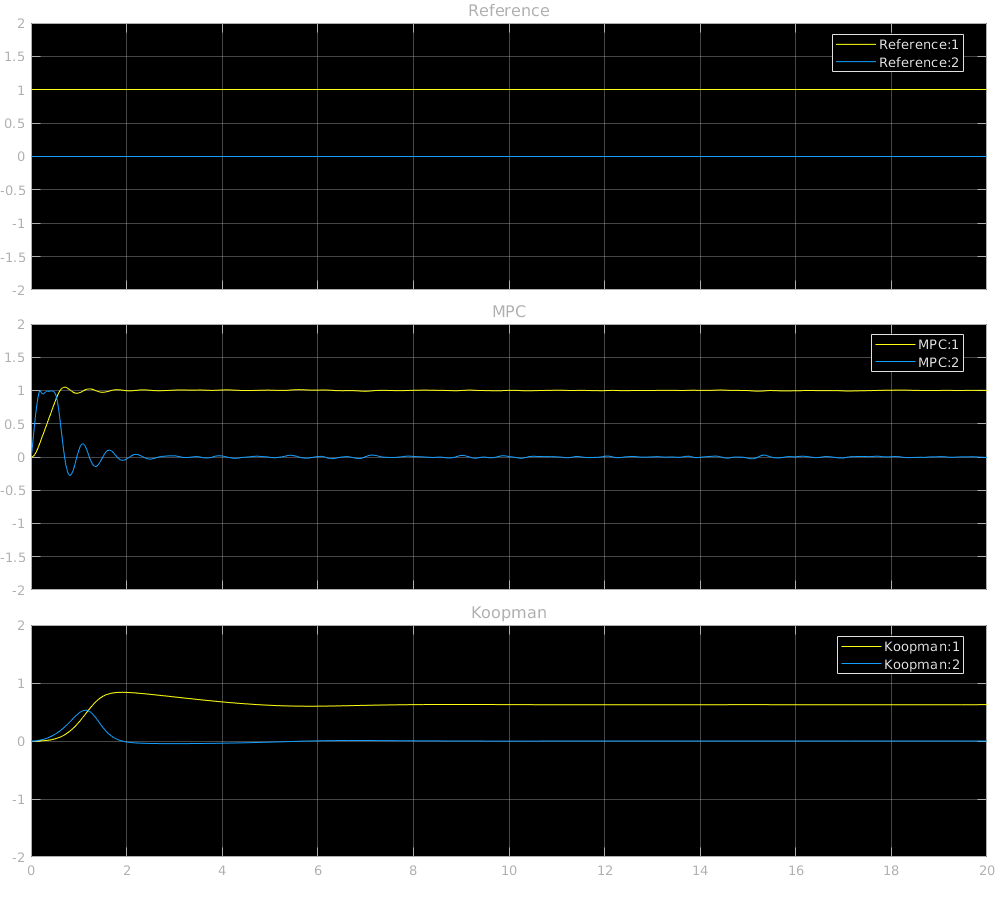
\includegraphics[width=\textwidth]{KK_10_Step.png}
            \caption{10 functions}
        \end{subfigure}
        \hfill
        \begin{subfigure}[b]{0.3\textwidth}
            \centering
            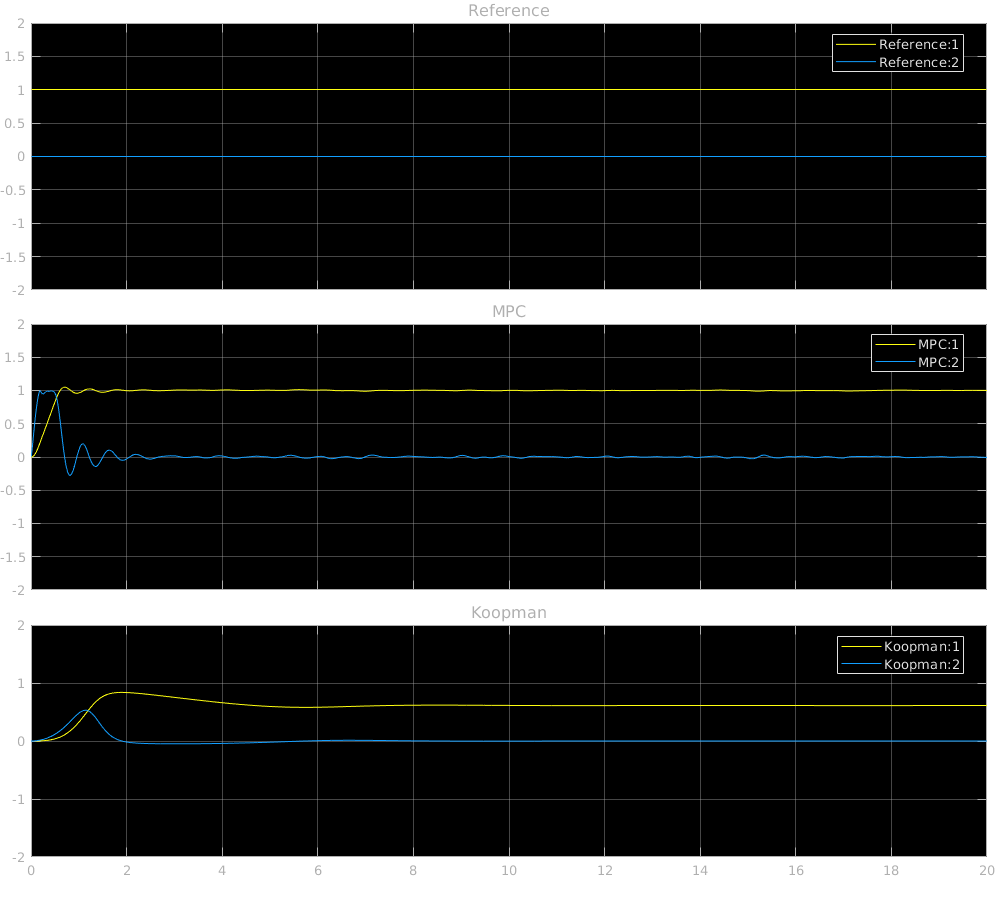
\includegraphics[width=\textwidth]{KK_20_Step.png}
            \caption{20 functions}
        \end{subfigure}
        \hfill
        \begin{subfigure}[b]{0.3\textwidth}
            \centering
            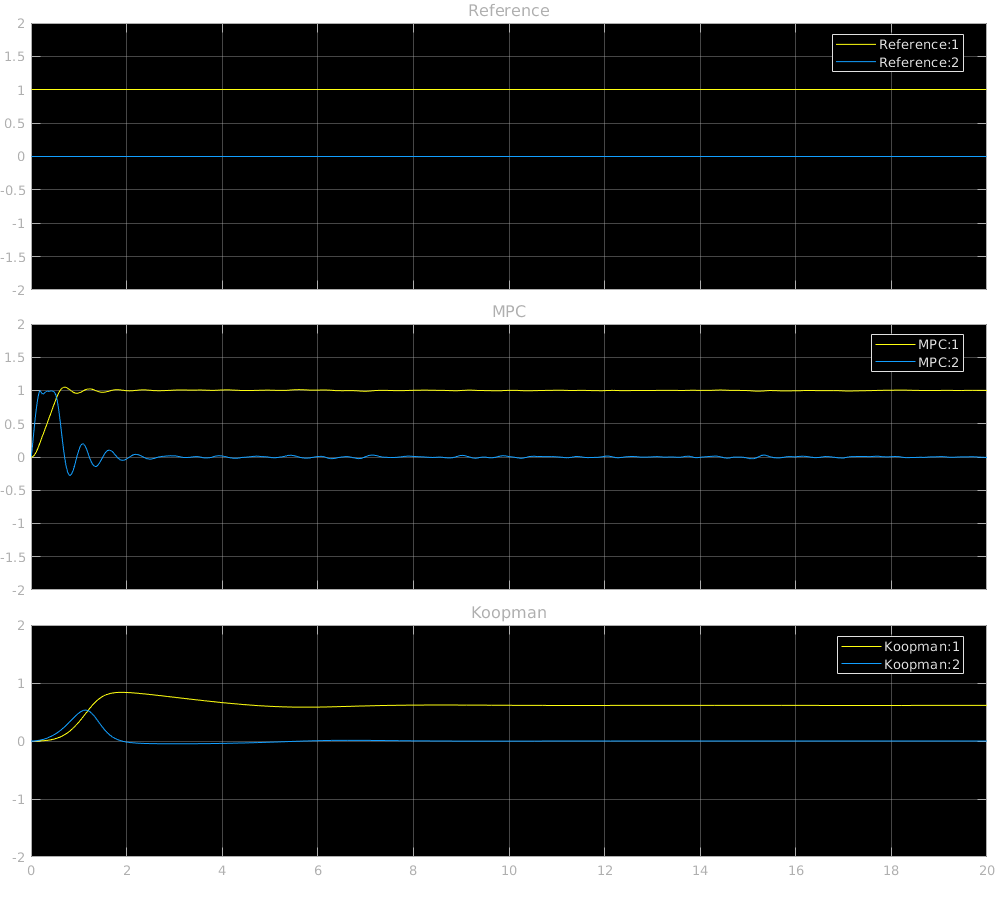
\includegraphics[width=\textwidth]{KK_50_Step.png}
            \caption{50 functions}
        \end{subfigure}
    \end{figure}
\end{frame}

\begin{frame}{Kalman-Koopman controller - Trajectory tracking}
    \begin{figure}
        \centering
        \begin{subfigure}[b]{0.3\textwidth}
            \centering
            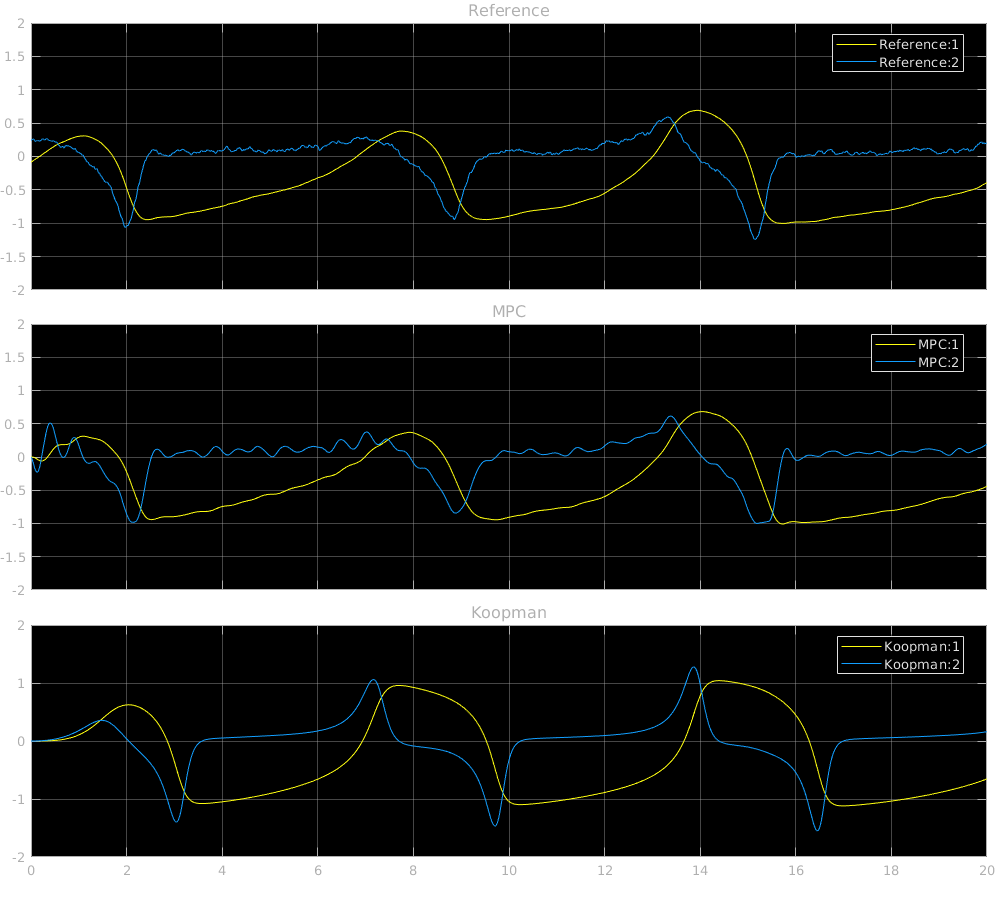
\includegraphics[width=\textwidth]{KK_10_Ref.png}
            \caption{10 functions}
        \end{subfigure}
        \hfill
        \begin{subfigure}[b]{0.3\textwidth}
            \centering
            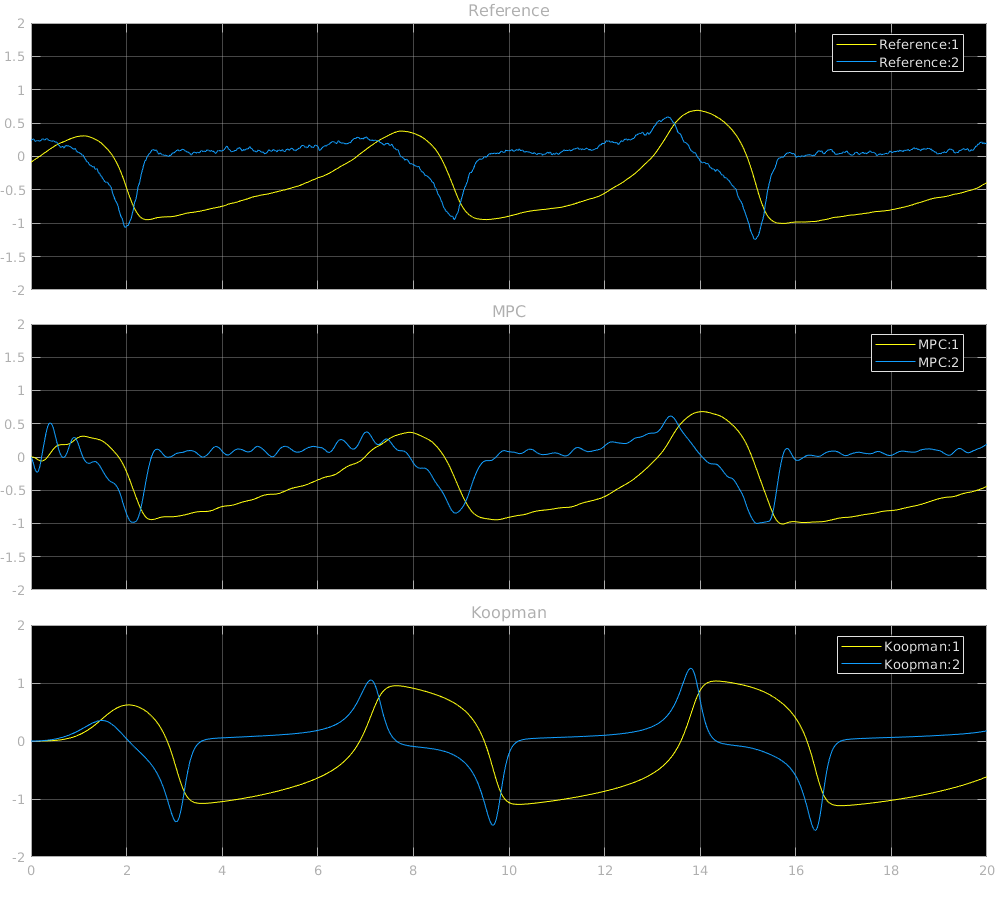
\includegraphics[width=\textwidth]{KK_20_Ref.png}
            \caption{20 functions}
        \end{subfigure}
        \hfill
        \begin{subfigure}[b]{0.3\textwidth}
            \centering
            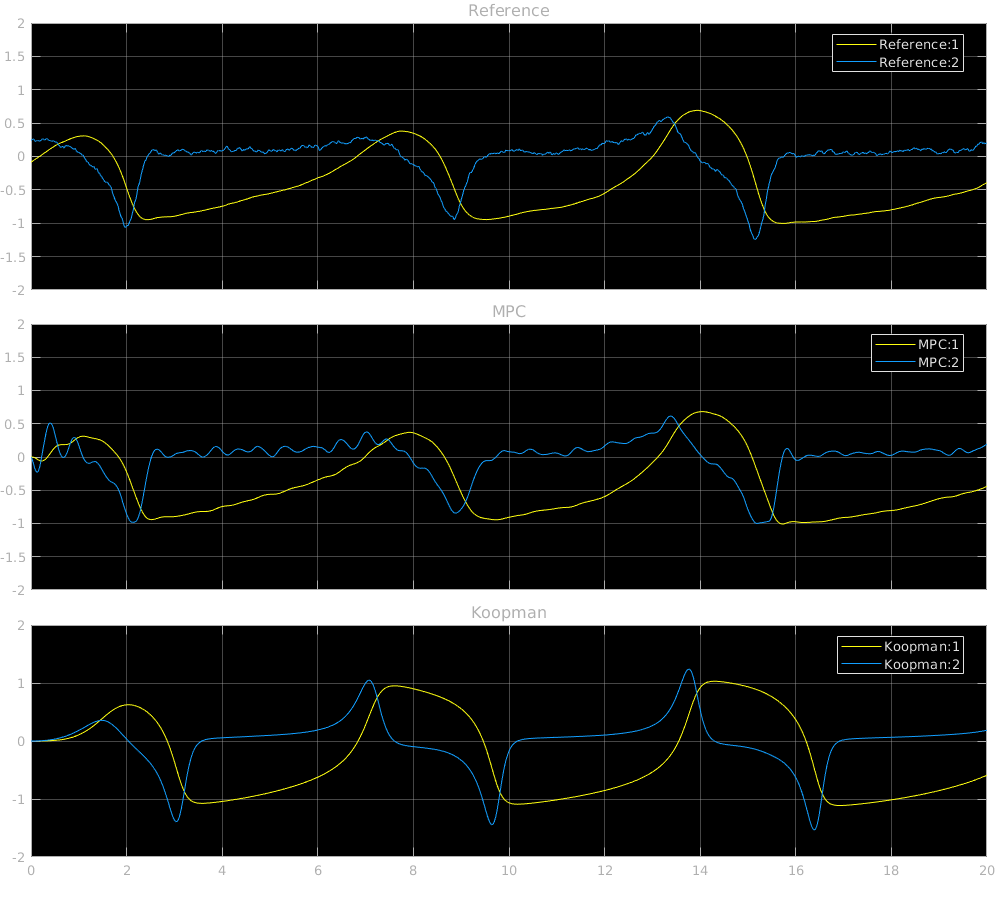
\includegraphics[width=\textwidth]{KK_50_Ref.png}
            \caption{50 functions}
        \end{subfigure}
    \end{figure}
\end{frame}

\end{document}